
\subsection{Merging Identical Object Code During Link Time}

The simplest way of merging identical functions is by looking at their object code, during link time.
\textit{Identical code folding}~(ICF) is an optimisation that identifies and merges two or more read-only sections, typically functions, that have identical contents.
This optimisation is commonly found in major linkers, such as \textit{gold}~\cite{tallam10,kwan12}, LLVM's \textit{lld}, and the MSVC linker~\cite{msvc-icf}.

Before applying ICS, it is a common practice for linkers to place functions in separate sections~\cite{tallam10,kwan12}.
Therefore, merging identical functions can be generalised to the problem of merging identical sections.
In the simplest case, two functions or sections are identical if they have exactly the same binary representation.
In general, two sections are considered identical if they have the identical section flags, data, code, and relocations.
Two relocations are considered identical if they have the same relocation types, values, and if they point to the same or, recursively, identical sections.

% Most object file formats, such as the \textit{Executable and Linkable Format} (ELF)~\cite{tallam10,kwan12}, are structured as separate sections of content, each section containing a certain type of content.
% The main types are code segment, different types of data segment, and relocation information.
% Relocation information describes how to modify other sections, connecting symbolic references to their definition.
% In other words, it assigns actual addresses for position-dependent code and data.
% For example, when a program calls a function, the associated call instruction must transfer control to the proper destination address at execution.

Once a set of identical functions have been identified, merging them requires a simple operation.
Only one of the functions in the set is kept for the final binary and all the other copies are discarded.
Afterwards, every reference to the discarded functions must be redirected to the kept function.
%We then map the symbols corresponding to the duplicate functions to have the same value as the symbol of the kept function.

% This is a trivial operation and the main challenge lies on the search strategy. 

% Figure~\ref{fig:icf-example} shows an example, adapted from Tallam~\etal~\cite{tallam10},
% of how generic programming in C++ can lead to identical functions in the object file.
% The C++ code in in Figure~\ref{fig:icf-example-code} presents
% a simple \textit{template class} and its member function being
% instantiated multiple times with different pointer types.
% Figure~\ref{fig:icf-example-object} shows the object code 
% targeting the Intel x86 architecture.
% For each instantiation of \textit{Foo}, a replica of its member
% function \textit{getElement} is created.
% Because the size of the different pointer types is the same,
% all replicas of \textit{getElement} are identical
% in the object file, which can be easily confirmed by
% comparing their binary representation. as shown in
% Figure~\ref{fig:icf-example-object}.

% \begin{figure}[h]
% \begin{tabular}{cc}
% \begin{subfigure}{.5\textwidth}
% 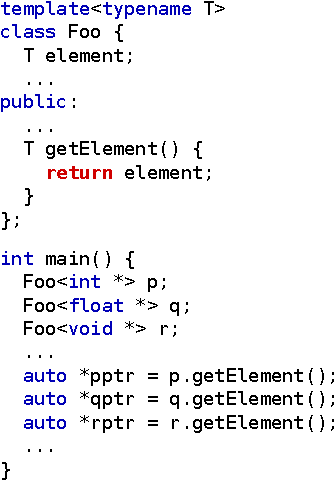
\includegraphics[scale=0.9]{src/relatedwork/figs/icf-example-1}
% \caption{A \textit{template class} with several instantiations.}
% \label{fig:icf-example-code}
% \end{subfigure} &
% \begin{subfigure}{.5\textwidth}
% 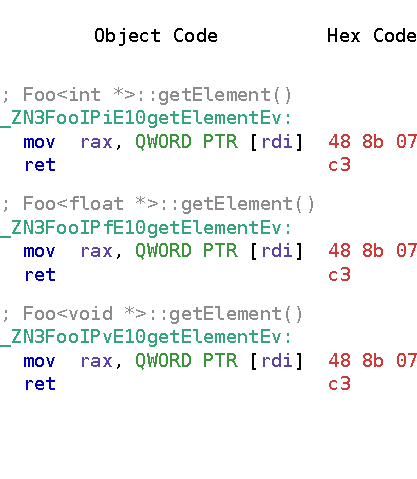
\includegraphics[scale=0.9]{src/relatedwork/figs/icf-example-2}
% \caption{Disassembled object file.}
% \label{fig:icf-example-object}
% \end{subfigure}
% \end{tabular}
% \caption{Example showing how a member function of a \textit{template class}
%   can produce code replication susceptible to \textit{identical code folding}.
%   For each instantiation of \textit{Foo}, a replica of the function
%   \textit{getElement} is created for the template instance.
%   When instantiated with pointer types, the object code of these functions will be identical.}
% \label{fig:icf-example}
% \end{figure}

Since the equality relation has a cyclic definition, ICF is defined as a fixed-point computation, i.e., it is applied repeatedly until a convergence is obtained.
There are two approaches with distinct trade-offs:
$(i)$ The pessimistic approach starts with all sections marked as being different and then repeatedly compare them trying to prove their equality, grouping those found to be identical, including their relocations.
This approach is implemented in the widely used \textit{gold} linker.
$(ii)$ The optimistic approach starts with all functions marked as potentially identical and then repeatedly compare trying to disprove their equality, partitioning those found to be different.
This approach is implemented in LLVM's linker, \textit{lld}.


% \subsection{The Pessimistic Algorithm}

% The pessimistic algorithm is implemented in the \textit{gold} linker.
% It starts by marking all functions as different and repeatedly compute their checksum to identify and merge more identical functions.
% This has the advantage that the algorithm can stop at any iteration, before the actual convergence, and correctness will be guaranteed.
% By limiting the number of iterations, regardless of convergence, we are essentially limiting the compilation-time overhead, potentially missing some optimisation opportunities.

% We can start with marking all functions as different and repeatedly do
% the checksumming.  This has the advantage that we do not need to wait
% for convergence. We can stop at any point and correctness will be
% guaranteed although not all cases would have been found.  However, this
% has a problem that some cases can never be found even if it is run until
% convergence.  Here is an example with mutually recursive functions :

% int funcA (int a)            int funcB (int a)
% {                            {
%   if (a == 1)                  if (a == 1)
%     return 1;                    return 1;
%    return 1 + funcB(a - 1);     return 1 + funcA(a - 1);
% }                            }

% In this example funcA and funcB are identical and one of them could be
% folded into the other.  However, if we start with assuming that funcA
% and funcB are not identical, the algorithm, even after it is run to
% convergence, cannot detect that they are identical.


% \subsection{The Optimistic Algorithm}

% The optimistic algorithm is implemented in LLVM linker, lld.

% \begin{figure}[h]

% \begin{subfigure}{\textwidth}
% \centering
% 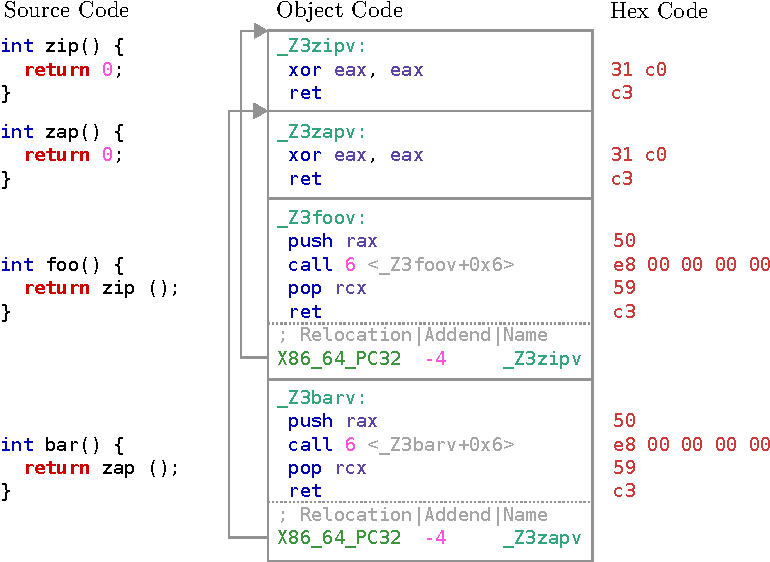
\includegraphics[width=0.9\textwidth]{src/relatedwork/figs/icf-example-code}
% \caption{.}
% \label{fig:identical-example-code}
% \end{subfigure}

% \begin{subfigure}{\textwidth}
% \centering
% 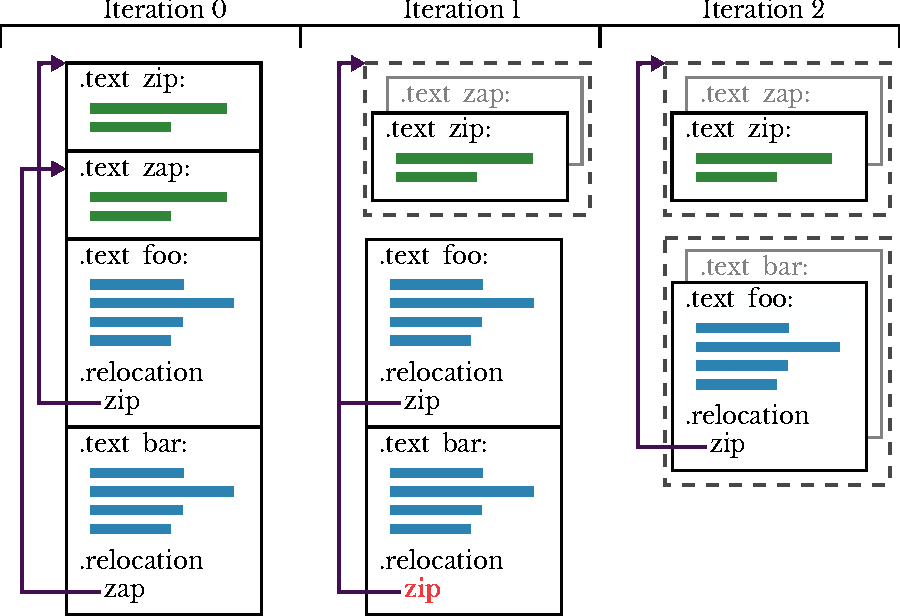
\includegraphics[width=0.9\textwidth]{src/relatedwork/figs/icf-example-diagram}
% \caption{.}
% \label{fig:identical-example-diagram}
% \end{subfigure}

% \caption{Example showing how a member function of a \textit{template class}
%   can produce code replication susceptible to \textit{identical code folding}.
%   For each instantiation of \textit{Foo}, a replica of the function
%   \textit{getElement} is created for the template instance.
%   When instantiated with pointer types, the object code of these functions will be identical.}
% \label{fig:icf-example}
% \end{figure}
